\documentclass{article}
\usepackage[utf8]{inputenc}
\usepackage{amsmath}
\usepackage{pst-all}
\usepackage{amssymb}
\usepackage{mathrsfs}
\usepackage[french]{babel}
\usepackage{graphicx}
\usepackage{titletoc}
\usepackage{hyperref}
\usepackage{amsthm}
\usepackage{pdfpages}
\usepackage{appendix}
\usepackage{MnSymbol}
\usepackage{fullpage}
\usepackage{url}
\usepackage{pgf,tikz,pgfplots}
\pgfplotsset{compat=1.15}
\usepackage{mathrsfs}
\usetikzlibrary{arrows}
\usepackage[inline]{asymptote}
\usepackage{pstricks}


% Environnements

\newtheorem{thm}{Théorème}[section]
\newtheorem{defn}[thm]{Définition}
\newtheorem{demo}[thm]{Démonstration}
\newtheorem{prop}[thm]{Proposition}
\newtheorem{lemme}[thm]{Lemme}
\newtheorem{rem}[thm]{Remarque}
\newtheorem{ex}[thm]{Exemple}
\newtheorem{cor}[thm]{Corollaire}
\newtheorem{corrige}[thm]{Corrigé}
\newtheorem{propr}[thm]{Propriété}
\newtheorem{conclu}[thm]{Conclusion}
\newtheorem{rappel}[thm]{Rappel}

 % Commande 
 
\newcommand{\Z}{\mathbb{Z}}
\newcommand{\N}{\mathbb{N}}
\newcommand{\R}{\mathbb{R}}
\newcommand{\C}{\mathbb{C}}
\newcommand{\F}{\mathbb{F}}
\newcommand{\Q}{\mathbb{Q}}
\newcommand{\Proj}{\mathbb{P}} % espace projectif

%Probabilités

\newcommand{\hyp}{\mathcal{H}}  %hypothèses


% Ensembles
\newcommand{\union}{\, \cup \,}     % union
\newcommand{\Union}{\, \bigcup \,}  % union (grand)
\newcommand{\inter}{\, \cap \,}     % intersection
\newcommand{\Inter}{\, \bigcap \,}  % intersection (grand)
%\newcommand{\sur}{\!\setminus\!}    % \ quotient d'ensembles


% Logique
\newcommand{\ou}{\text{ ou }}   % ou
\newcommand{\et}{\text{ et }}   % et
\newcommand{\non}{\text{non+}}    % non 
\newcommand{\avec}{\text{ avec }} %avec
\newcommand{\sinon}{\text{ sinon }} %sinon


% Parenthèses etc
\newcommand{\pars}[1]{\ensuremath{\left( #1 \right)}}               % (*) parenthèses
\newcommand{\set}[1]{\ensuremath{\left\{ #1 \right\}}}              % {*} ensemble
\newcommand{\braces}[1]{\ensuremath{\left\{ #1 \right\}}}           % {*} synonyme de \set
\newcommand{\abs}[1]{\ensuremath{\left| #1 \right|}}                % |*| valeur absolue/module
\newcommand{\norm}[1]{\ensuremath{|| \overrightarrow{#1} ||}}             % ||*|| norme vectorielle
\newcommand{\scal}[1]{\ensuremath{\left\langle #1 \right\rangle}}   % <*> produit scalaire
\newcommand{\ve}[1]{\ensuremath{\overrightarrow{#1}}}               % vecteur
\newcommand{\entiers}[1]{\ensuremath{\left[\!\left[ #1 \right]\!\right]}} % [|*|] intervalle d'entiers
\newcommand{\vect}[1]{\overrightarrow{#1}}



% Analyse
\newcommand{\eps}{\varepsilon}      % le "joli" epsilon
\newcommand{\D}{\operatorname{d}}     % d (droit)
\newcommand*{\seq}[2][0]{\ensuremath{\pars{#2}_{n \ge #1}}}     % suite (*)_{n ≥ 0}, on peut changer le 0 en argument optionnel
\newcommand*{\series}[2][0]{\ensuremath{\sum_{n \ge #1} #2}}    % série ∑_{n ≥ 0} *, on peut changer le 0 en argument optionnel
\newcommand*{\infsum}[2][0]{\ensuremath{\sum_{n \ge #1}^{\infty} #2}}   % somme infinie ∑_{n ≥ 0}^∞ *, on peut changer le 0 en argument optionnel
\newcommand{\goesto}[1][n \to \infty]{\ \underset{#1}{\longrightarrow} \ } % tend vers : --> x->0
\newcommand{\supe}[1]{\underset{#1}{\operatorname{sup}}}
\newcommand{\mini}[1]{\underset{#1}{\operatorname{min}}}
\newcommand{\infi}[1]{\underset{#1}{\operatorname{inf}}}
\newcommand{\maxi}[1]{\underset{#1}{\operatorname{max}}}
\newcommand{\norme}[2]{||#1||_{#2}}



% Trigo hyperbolique
\newcommand{\ch}{\operatorname{ch}}
\newcommand{\sh}{\operatorname{sh}}
\newcommand{\tah}{\operatorname{th}}
\newcommand{\cosinus}[1]{\operatorname{cos} \left( #1 \right)} %%%%%%%
\newcommand{\sinus}[1]{\operatorname{sin} \left( #1 \right)}

% Algèbre linéaire
\newcommand{\mat}[1]{\ensuremath{\pars{\begin{matrix} #1 \end{matrix}}}} % (**) matrice
\newcommand{\Det}{\operatorname{Det}} % Det (majuscule, \det existe déjà)
\newcommand{\diag}{\operatorname{diag}}
\newcommand{\Id}{\operatorname{Id}}


% Arithmétique
\newcommand{\legendre}[2]{\ensuremath{\left(\frac{#2}{#1}\right)}} % Symbole de Legendre
\newcommand{\Gal}{\operatorname{Gal}}


% Complexes
\newcommand{\re}{\operatorname{Re}}
\newcommand{\im}{\operatorname{Im}}


% Groupe de Lie, représentations
\newcommand{\Oronde}{\mathcal{O}}
\newcommand{\Hecke}{\mathcal{H}}
\newcommand{\Ind}{\operatorname{Ind}}
\newcommand{\GL}{\operatorname{GL}}
\newcommand{\SL}{\operatorname{SL}}
\newcommand{\Hom}{\operatorname{Hom}}
\newcommand{\End}{\operatorname{End}}
\newcommand{\Aut}{\operatorname{Aut}}
\newcommand{\Spec}{\operatorname{Spec}}
\newcommand{\Vect}{\operatorname{Vect}}
\newcommand{\Supp}{\operatorname{Supp}}
\newcommand{\ssi}{\Longleftrightarrow}  

% Déprécié
\newcommand{\GUE}{\operatorname{GUE}} % Déprécié
\newcommand{\dt}{\,.\,}

%Physique opérateur mathématiques
\newcommand{\grad}{\overrightarrow{\nabla}} %gradient avec fleche
\newcommand{\diver}[1]{\overrightarrow{\nabla}.\overrightarrow{#1}} %divergence
\newcommand{\rot}[1]{\overrightarrow{\nabla} \wedge \overrightarrow{#1}} %rotationnel
\newcommand{\df}[2]{\frac{\partial{#1}}{\partial #2}} %derivee partielle
\newcommand{\ddf}[2]{\frac{\partial^2{#1}}{\partial #2^2}} %derivee partielle seconde
\newcommand{\lap}[1]{\nabla^2 \ve{#1}} %laplacien 


%somme et produit
\newcommand{\somme}[2]{\overset{#2}{\underset{#1}{\sum}}} 
\newcommand{\produit}[2]{\overset{#2}{\underset{#1}{\Pi}}} 


%limite
\newcommand{\tendvers}[2]{\underset{#1 \rightarrow #2}{\longrightarrow}} %tend vers
\newcommand{\limite}[2]{\underset{#1 \rightarrow #2}{\operatorname{lim}}} %limite

\newcommand{\poubelle}[1]{} %fonction poubelle prend quelque chose en argument mais ne renvoie rien 

%physique
\newcommand{\cste}{\operatorname{cste}} %constante
\newcommand{\moy}[1]{\left< #1 \right>}  %valeur moyenne
\newcommand{\U}[1]{\vect{u}_{#1}}

\parindent0pt %retirer l'indentation



\date{Le 27 Mai 2020}
\begin{document}
\newpage

\title{\Huge{Rapport de projet de simulation numérique \\ \textbf{Malin comme un...blob\\}
}}
\vspace{0.5cm}


\maketitle


\begin{center}
    \rule{0.9\linewidth}{0.5pt}\\
        \vspace{5mm}
        Groupe 4\\ 
        \ \\
	    ALQUIER Rodolphe\\
      BALANNEC Ancelin\\
      CAVALIER Pierre\\
      CONTENTIN Théo\\
      HARDY Paul\\
	    \ \\
		Université Paris-Saclay\\
		L2 Double Licence Maths-Physique\\
        \vspace{5mm}	
\rule{0.9\linewidth}{0.5pt}
\vspace{0.5cm}
\end{center}
\begin{center}
\title{\Huge\textbf{{Los Commandos}}}
\end{center}

\begin{center}
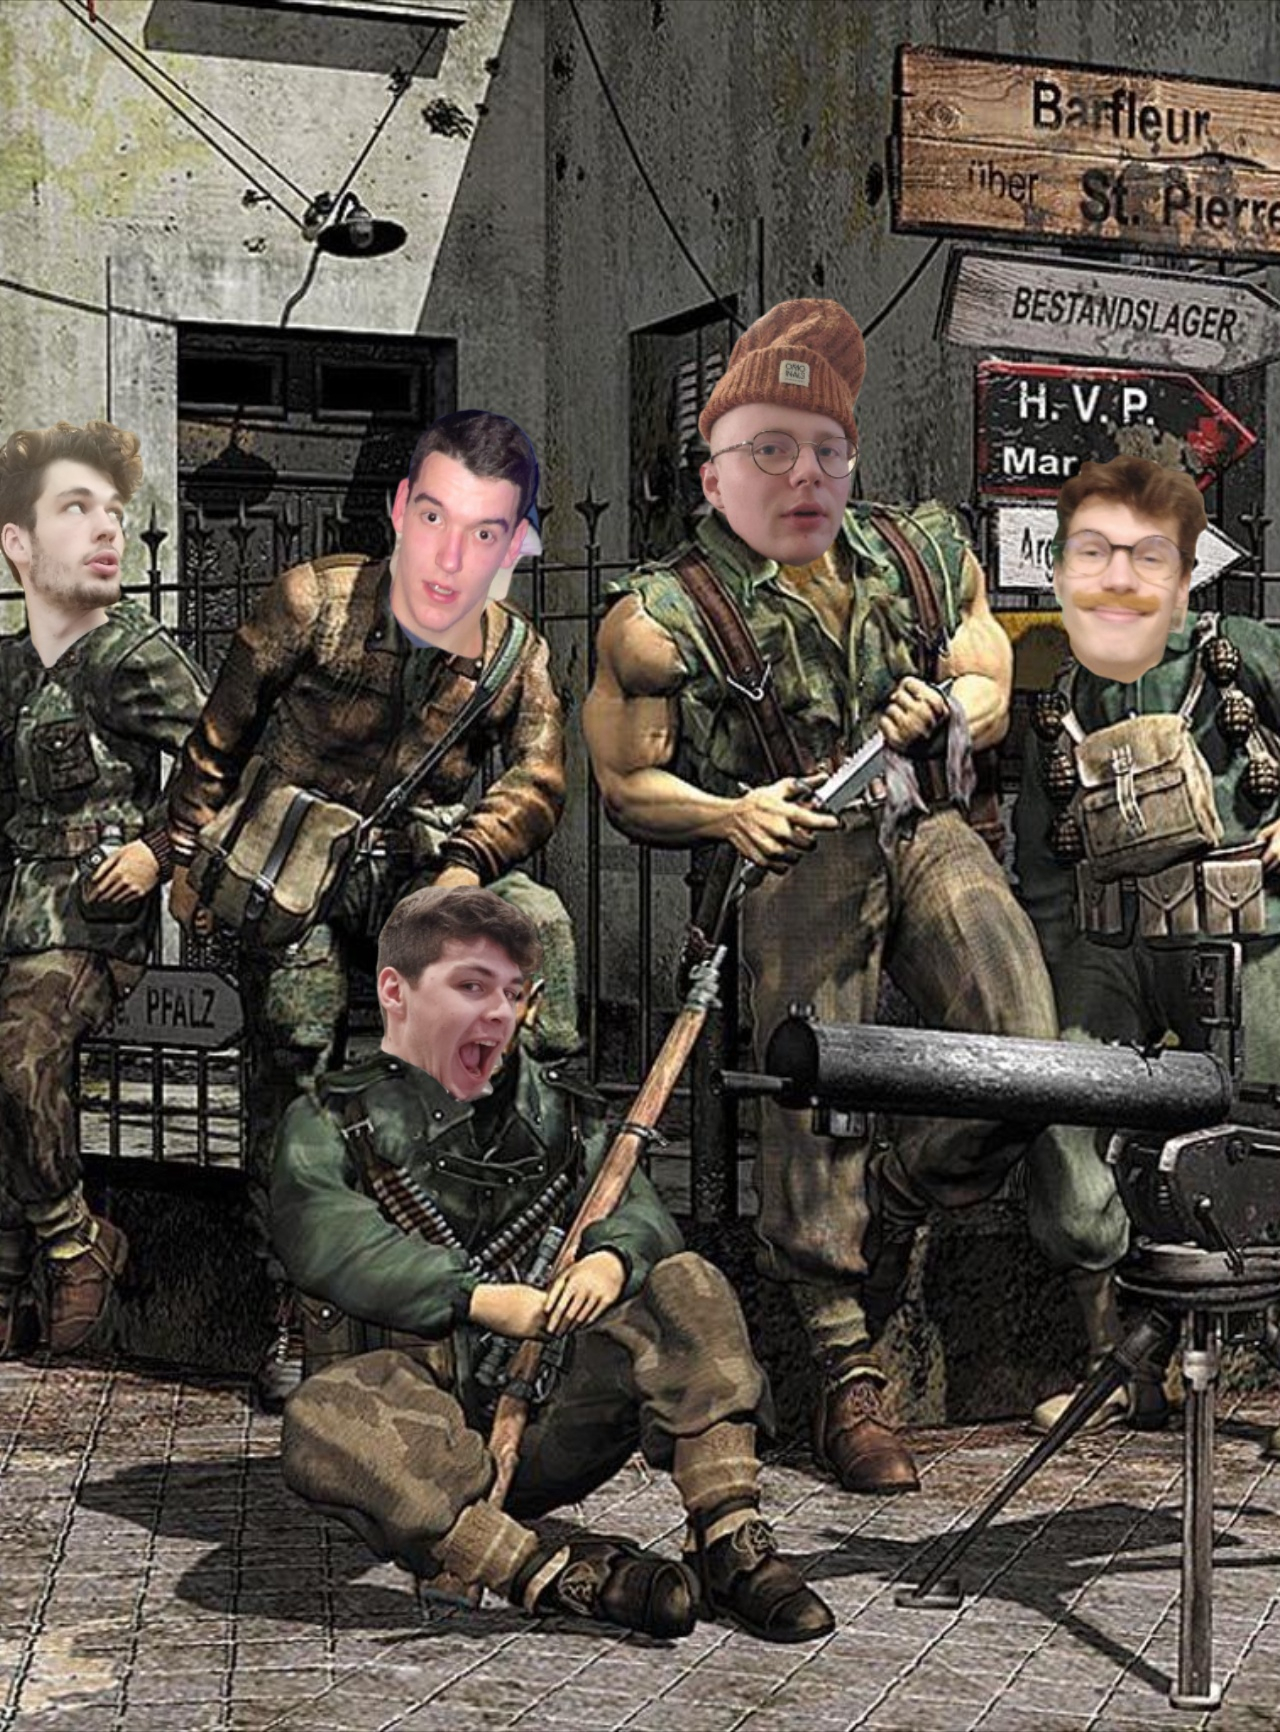
\includegraphics[width=6cm]{Los_commandos.jpg}
\end{center}


\begin{document}
\maketitle
\newpage
\tableofcontents
\newpage
\section{\Large{\texbf{Introduction}}}
\hspace*{1cm} Durant ce projet, nous avons travaillé sur "le blob"; cet organisme unicellulaire qui peut croître de plusieurs centimètre par heure et devient donc une cellule macroscopique. Le \textit{Physarum polycephalum}, de son vrai nom, peut créer des structures internes, des ramifications permettant d'acheminer la nourriture des sources aux puits. Dans un premier temps nous avons considéré ces puits et sources comme fixés à des noeuds respectifs, puis dans un second temps, nous avons considéré que ces derniers pouvait changer de positions au cours du temps. Pour identifier les sommets, nous les avons numérotés de $0$ à $N-1$ avec $N$ le nombre total de points (N est un carré d'entier pour le maillage rectangulaire) de cette manière :

\begin{center}
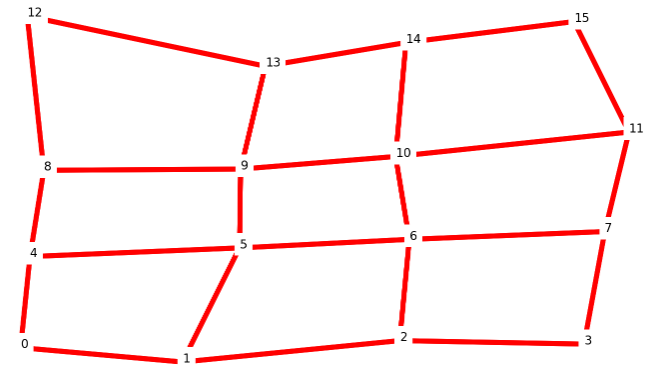
\includegraphics[width=12cm]{arrangement.png}
\end{center}

\\

\section{Présentation du modèle}
\hspace*{1cm} On  suppose  qu’à l'état initial  le  blob  est  un  réseau  de  N  noeuds  tous  ́equivalents numerotés  de 0 à N. Ces noeuds sont reliés entre eux par des branches dans lesquelles circuleront les nutriments. Les branches ont des longueurs et diamètre variables . Le débit $Q_{ij}$ dans la branche reliant le noeud i au noeud j est donne par la loi de Poiseuille :

$$ Q_{ij} = \frac{\pi r^{4}}{8 \eta L_{ij}} (p_{j} - p_{i}) = \frac{D_{ij}}{L_{ij}} (p_{j} - p_{i}) $$


où,$L_{ij}$ est la longueur de la branche , $\eta$ est la viscosité du liquide,$p_{j}$ et $p_{i}$ les pressions au niveau des noeuds j et i. Au niveau du noeud i, le débit est positif lorsque le fluide va vers celui-ci. Comme la viscosité est la même partout, on introduit la conductivité ${D_{ij}$ .\\
Si le noeud k est une source, $\somme{j}{}Q_{kj}=I_{k} < 0$.  Ici $I_{k}$ est  le  débit  total  sortant  du  noeud . De même, si le noeud l est un puits , $\somme{j}{}Q_{lj}=I_{l} >0$. Pour les autres noeuds i, la conservation du debit s’ecrit : $\somme{j}{}Q_{ij}=I_{i}=0$.\\
Enfin, tout ce qui rentre dans le reseau doit en resortir. Ceci conduit à la relation :$\somme{k}{}I_{k}+\somme{l}{}I_{l}= 0$.\\
\ \\
On remarque qu’il est possible de déterminer les pressions $p_{i}$ de tous les noeuds en résolvant le système de N ́equations à N inconnues,  $AP=I$ avec A est une matrice ($N\times N$), P un vecteur à N dimensions dont la composante i est la pression $p_{i}$ , et I est un vecteur à N dimensions dont chaque composante i est le débit total $I_{i}$ au niveau du noeud i.\\
En résolvant ce système on obtient toutes les pressions, et ainsi on peut calculer les débits $Q_{ij}$ dans chaque branche reliant le noeud i et j.\\
\ \\
Le rayon r de chaque branche  ́evolue au cours du temps.Il tend à diminuer avec le temps. En revanche si un débit $Q_{ij}$  non nul s’écoule dans la branche, son rayon est non seulement stabilisé,mais il sera d’autant plus grand que le débit sera  ́elevé (jusqu’à un certain point).\\
La conductivité $D_{ij}$ ́evolue avec le temps t de la manière suivante :
$$\frac{dD_{ij}}{dt}=f(Q_{ij})-\frac{D_{ij}}{\tau}$$

Avec $\tau$ , le temps caractéristique de disparition d’une branche et f une fonction modélisant la réponse de la branche au débit la traversant :
$$f(Q)=\frac{|Q|^{\gamma}}{1+|Q|^{\gamma}}$$
Et pendant un temps dt nous obtenons :
$$D_{ij}(t+dt)\approx D_{ij}(t)+(f(Q_{ij})-\frac{D_{ij}}{\tau})dt$$


\section{Résolution mathématique AP = I}
\hspace*{1cm} Comme expliqué ci-dessus on cherche la matrice A qui nous permettra d'obtenir P la matrice correspondant aux pressions de chaque nœud.\\
\begin{equation}
\begin{pmatrix}
    a_{11} & \cdots & a_{1N} \\ 
    \\  
    \vdots & \ddots & \vdots \\ 
    \\
    a_{N1} & \cdots & a_{NN}
    \end{pmatrix}
    \times
\begin{pmatrix} p_{1} \\ 
                \\
                \vdots \\ 
                \\ 
                p_{N}
                \end{pmatrix}
    =
\begin{pmatrix} I_{1} \\ 
                \\
                \vdots \\ 
                \\  
                I_{N}
                \end{pmatrix} \end{equation}
\\

Où

\\

\begin{equation} I_{i} = \somme{\text{j}}{} Q_{ij} \end{equation}

\\
Or $Q_{ij}$ est nul si i et j ne sont pas voisins, on note ainsi $V[i]$ le voisinage de I
\\
\begin{equation} I_{i} = \somme{j\in V[i]}{}\frac{D_{ij}}{L_{ij}} (p_{j} - p_{i}) \end{equation}

On obtient finalement :


\begin{equation} a_{ij} = \begin{cases}
\somme{j\in V[i]}{}\frac{D_{ij}}{L_{ij}} \hspace*{0.433cm} \text{si} \hspace*{0.1cm} \text{j = i} \\
\\  %Enlever le "\\" de cette ligne pour enlever l'espace sur le pdf
\frac{D_{ij}}{L_{ij}} \hspace*{1.25cm} \text{si} \hspace*{0.1cm} \text{j}\in \text{V[i]} \\
\\ %Enlever le "\\" de cette ligne pour enlever l'espace sur le pdf
0 \hspace*{1.625cm} \text{si} \hspace*{0.1cm} \text{j} \not\in \text{V[i]}
\end{cases}\end{equation}
\\

Dans notre cas, la matrice A est de rang $N-1$ et pour résoudre ce système, on utilise la méthode des moindres carrés avec le module \textbf{np.linalg.lstsq} de numpy.

\section{Résolution informatique}

Pour répondre au problème qui nous a été posé nous avons travaillé avec deux classes, une pour les noeuds du réseau et une pour le blob en lui même.\\

Cette classe nous permet de répertorier toutes les informations sur un nœud. À un point $n$ on associe ses coordonnés $x$ et $y$ et une légère fluctuation dans un carré de côté 1 et de centre le point. À ce point, on associe sa liste de voisins (create$\_$voisins) et à partir de cette dernière on obtient la distance (get$\_$L) et la conductivité (get$\_$D) par rapport à ses voisins.\\

À partir de cette classe nous avons créer la classe blob qui génère tout le maillage avec des options qui permettent différents type de maillage and qu'une répartitions des puits et des sources aussi bien fixes que mobiles. De plus cette classe initialise aussi les paramètres des nœuds ainsi que l'intensité des sources et des puits.\\

De plus nous avons rajouté une fonction pour répresenter graphiquement chaque partie du blob (plot), que ce soit les nœud (plot$\_$noeud), les branches (plot$\_$branch), les puits (plot$\_$puits), les sources (plot$\_$sources). Nous avons ajuté une fonction (get$\_$noeud) qui renvoie l'objet nœud correspondant à l'indice n donné, ainsi que des fonctions calculant la matrice A comme vu précedemment dans la partie 3, d'obtenir l'intensité (get$\_$I) en un nœud et de calculer la pression (calcule$\_$p) en pour un nœud donné\\

Ensuite nous avons la fonction qui permet d'avancer à l'instant $t + dt$, à partir des données à l'instant t 


\end{document}

